%Organize this section according to the rules defined in the project description. 


\subsection{External Interface Requirements}
    \subsubsection{User Interfaces}
    We prefer not to tie our design to any guidelines so early in the project so we will probably give some snippet of the user interfaces in the Design Document. However the principles who will guide our design will be clearness and minimalism. We believe that at the basis of well working web application there must be a nice user interface. We are also convinced that being minimal and simple looking is a plus for a web application since a confusing user interface is one of the biggest reason why users dislike a certain website and prefer another to it.

    \subsubsection{Hardware Interfaces}
    Being our project a web application there are not many hardware requirements. From the client side perspective the only request is about the size of the monitor. Indeed the website is going to be developed for desktop view exclusively. Apart of that any laptop with a stable internet access will suffice. On the server side any kind of is okay since our website does not have any particular need for any kind of special computing power or similar things.

    \subsubsection{Software Interfaces}
    From the point of view of software interfaces there are some more requests but still pretty standard ones. Here is the list of the software interfaces needed:
    \begin{enumerate}
        \item  \textbf{Browser Compatibility}: the platform must be compatible with all last stable versions of major web browsers
        \item \textbf{Email Service Provider}: to send automatic emails to confirm accounts creation and registration
    \end{enumerate}
    \subsubsection{Communication Interfaces}
    Apart of the email confirmation system, discussed in the section above on Software Interface, S\&C communicates important information to users through notifications on the website.
    \begin{enumerate}
        \item  \textbf{Push Notifications}: notifications created when a company posted an internship or a student with right skill set for an internship becomes available on the platform
        \item \textbf{Real Time Notifications}: notifications created when an action is performed by a user to let him/her know that it has been successful or not
    \end{enumerate}
\subsection{Functional Requirements}
    The listed requirements are in the form suggested by IEEE\cite{502838}: 
    \newline
    \newline
    [Condition][Subject][Action][Object][Constraints on the Action]
    \subsubsection*{Users:}
        \begin{enumerate}[label=\textbf{R\arabic*}]
            \item S\&C shall allow users to sign up.                  
            \item S\&C shall allow users to confirm their mail        
            \item S\&C shall allow users to log in.                   
            \item S\&C shall allow users to log out.                  
            % US DONE
            \item S\&C shall allow users to update their profile information.      
            \item S\&C shall allow users to examine internship positions.
            \end{enumerate}
        
    \subsubsection*{Students:}
        \begin{enumerate}[label=\textbf{R\arabic*},resume]
            \item After they registered and confirmed their email, S\&C shall allow students to upload their CV.  
            \item After they registered and confirmed their email, S\&C shall allow users to fill the required information (Phone number, Degree program, etc).
            \item S\&C shall allow students to search for a specific kind of internship.  
            \item S\&C shall allow students to apply for an internship.                    
            \item If an internship position suited to a student is opened, S\&C shall notify the student
            \item When a student issues a search for an internship, S\&C shall list the different positions aligned with the student's profile.         
    
            
        \end{enumerate}
    
    \subsubsection*{Applications:}
        \begin{enumerate}[label=\textbf{R\arabic*},resume]
            \item If an application has been accepted by a company, S\&C shall allow the student who made the application to confirm or refuse the internship
            \item If a company signals that it needs a quiz of the students' skills, S\&C shall allow the student to schedule the quiz
            \item After a quiz has been scheduled, S\&C shall allow the student to take the quiz
            \item If a company signals that it needs an interview to test the students' skills, S\&C should allow the student and the company to schedule the interview
            \item After the interview has been scheduled, S\&C should allow the student to access the link of the virtual room
            \item S\&C shall allow the student to see the status of its applications
            
        \end{enumerate}
    
    \subsubsection*{Companies:}
        \begin{enumerate}[label=\textbf{R\arabic*},resume]
            \item After they registered and confirmed their email, S\&C shall allow companies to fill the required information (Name, Surname, etc).
            \item S\&C shall allow companies to open internship positions.
            \item S\&C shall allow companies to close internship positions.
            \item If an a new profile of a student with a CV who could interest a company becomes available on the platform, S\&C shall notify the company
        \end{enumerate}
    
    \subsubsection*{Communication during the internship:}
         \begin{enumerate}[label=\textbf{R\arabic*},resume]
            \item S\&C shall allow companies to leave private notes to students who are carrying out an internship with it
            \item S\&C shall allow companies to send news about the internship to students who are carrying it out
            \item S\&C shall allow both parties to communicate problems in a specific space of the website
        \end{enumerate}
    
    \subsubsection*{Feedback and Suggestions:}
        \begin{enumerate}[label=\textbf{R\arabic*},resume]
            \item S\&C shall allow students who took an internship with a company to rate the internship and vice versa
            \item S\&C shall allow students who took an internship with a company to give suggestions to the company and vice versa
            \item S\&C shall allow companies to send news about the internship to students who are carrying it out
            \item S\&C shall allow both parties involved in an internship to communicate problems in a dedicated space
        \end{enumerate}
        \subsubsection*{Universities:}
        \begin{enumerate}[label=\textbf{R\arabic*},resume]
            \item After they registered and confirmed their email, S\&C shall allow universities to complete their profile by filling the required field
            \item S\&C shall allow universities to monitor the status of the internship of their students
            \item S\&C shall allow universities to see details of the internship of their students
        \end{enumerate}
        
\newpage

\subsection{Use Cases and Use Case Diagrams}

    \subsubsection{User Use Cases}
    
        \begin{enumerate}[label=\textbf{[US\arabic*]}, left = 0pt, align = left]
            % -- US1 --                                                      
            \item \textbf{User Login}
            
            \begin{longtable}{|l|p{11cm}|}  
                \hline
                \textbf{Name} & 
                    \textbf{User Login} \\
                \hline
                
                \textbf{Actors} & 
                    \begin{enumerate}[label=\textbullet, itemsep=0em]
                        \item User;
                        \item S\&C System.
                    \end{enumerate} \\
                \hline
                
                \textbf{Entry Condition} & 
                    \begin{enumerate}[label=\textbullet, itemsep=0em]
                        \item The user wants to log in;
                        \item The user has an account and is on the main page of S\&C.
                    \end{enumerate} \\
                \hline
                
                \textbf{Event Flow} &
                    \begin{enumerate}[label=\arabic*., itemsep=0.2em]
                        \item The user presses the "Login" button;
                        \item S\&C redirects the user to the login page;
                        \item The user types the Email in the corresponding form field;
                        \item The user types the password in the corresponding form field;
                        \item The user presses the "Log in" button;
                        \item S\&C validates the data;
                        \item S\&C redirects the user to the homepage of S\&C.
                    \end{enumerate} \\
                \hline
                
                \textbf{Exit Condition} & 
                    The user logs into his/her profile. \\
                \hline
                
                \textbf{Exceptions} &
                    \begin{enumerate}[label=\arabic*., itemsep=0.1em]
                        \item A user with the entered email doesn't exists.
                            \begin{itemize}[label=\textbullet, itemsep=0em]
                                \item In that case, S\&C will display an error message on the screen.
                            \end{itemize}
                        \item The entered password and the stored password do not match.
                            \begin{itemize}[label=\textbullet, itemsep=0em]
                                \item In that case, S\&C will display an error message on the screen.
                            \end{itemize}
                    \end{enumerate} \\
                \hline
                
            \end{longtable}

            \newpage 
            \begin{figure}[h!]
                \centering
                    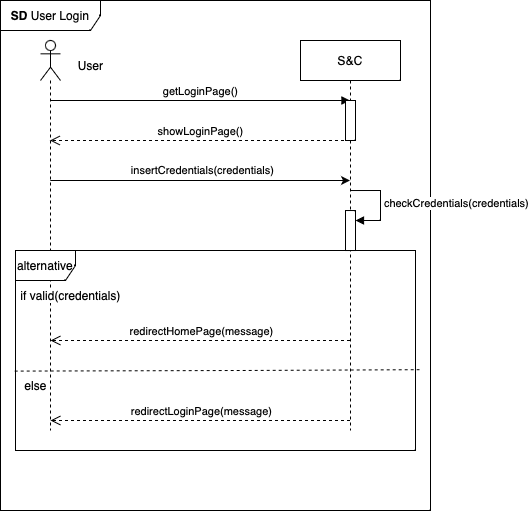
\includegraphics[width=1\textwidth]{RASD/Images/UseCases/US01_UserLogin.drawio.png}
                \label{fig:example}
            \end{figure}
  
            % -- US2 --                                                     
            \newpage
            \item \textbf{User Logout}
            
            \begin{longtable}{|l|p{11cm}|}  
                \hline
                \textbf{Name} & 
                    \textbf{User Logout} \\
                \hline
                
                \textbf{Actors} & 
                    User \\
                \hline
                
                \textbf{Entry Condition} & 
                    \begin{enumerate}[label=\textbullet, itemsep=0em]
                        \item The user wants to log out;
                        \item The user has an account, is logged in, and is on his/her homepage.
                    \end{enumerate} \\
                \hline
                
                \textbf{Event Flow} &
                    \begin{enumerate}[label=\arabic*., itemsep=0.2em]
                        \item The user presses the "Logout" button;
                        \item S\&C displays a Success Message;
                        \item S\&C redirects the user to the main page;
                    \end{enumerate} \\
                \hline
                
                \textbf{Exit Condition} & 
                    The user logs out his/her profile. \\
                \hline
                
                \textbf{Exceptions} &
                    \begin{enumerate}[label=\arabic*., itemsep=0.1em]
                        \item The user doesn't have an account.
                            \begin{itemize}[label=\textbullet, itemsep=0em]
                                \item In that case, S\&C will display an error message on the screen.
                            \end{itemize}
                    \end{enumerate} \\
                \hline
                
            \end{longtable}

            \begin{figure}[h!]
                \centering
                    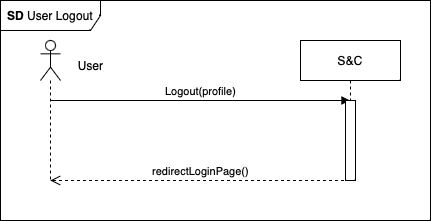
\includegraphics[width=1\textwidth]{RASD/Images/UseCases/UserLogout.drawio.png}
                \label{fig:example}
            \end{figure}

            % -- US3 --                                                      
            \newpage
            
            \item \textbf{Update User Profile}
            
            \begin{longtable}{|l|p{11cm}|}  
                \hline
                \textbf{Name} & 
                    \textbf{Update User Profile} \\
                \hline
                
                \textbf{Actors} & 
                    User \\
                \hline

                \textbf{Entry Condition} & 
                    \begin{enumerate}[label=\textbullet, itemsep=0em]
                        \item The user decides to modify his/her profile;
                        \item The user has an account, is logged in, and is on his homepage.
                    \end{enumerate} \\
                \hline
                
                \textbf{Event Flow} &
                    \begin{enumerate}[label=\arabic*., itemsep=0.2em]
                        \item The user presses the "Edit Profile" button;
                        \item S\&C redirects the user to the personal profile page;
                        \item The user choose which information modify;
                        \item The user presses the "Modify" button on the right of the desired category;
                        \item The user modifies the data;
                        \item The user presses the "Apply Changes" button;
                        \item S\&C validates the data;
                        \item S\&C redirects the user to the homepage of S\&C.
                    \end{enumerate} \\
                \hline
                
                \textbf{Exit Condition} & 
                    The user's profile is successfully updated and saved in the system. \\
                \hline
                
                \textbf{Exceptions} &
                    \begin{enumerate}[label=\arabic*., itemsep=0.1em]
                        \item Missing Required Fields:
                            \begin{itemize}[label=\textbullet, itemsep=0em]
                                \item If any mandatory fields are left empty, S\&C will display an error message.
                            \end{itemize}
                        \item Invalid Data Format:
                            \begin{itemize}[label=\textbullet, itemsep=0em]
                                \item If at least one data is invalid, an error message is displayed;
                            \end{itemize}     
                    \end{enumerate} \\
                \hline
                
            \end{longtable}
        
            \newpage
            \begin{figure}[h!]
                \centering
                    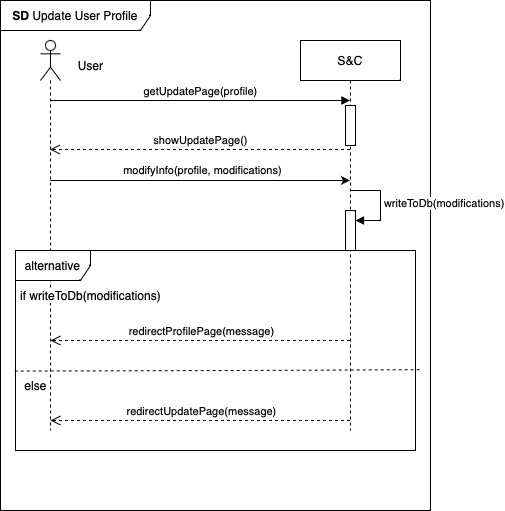
\includegraphics[width=1\textwidth]{RASD/Images/UseCases/UserUpdate.drawio.png}
                \label{fig:example}
            \end{figure}

        \end{enumerate}

    % -----------------------------------
    \newpage
    \subsubsection{Student Use Cases}
    
        \begin{enumerate}[label=\textbf{[US\arabic*]}, left = 0pt, align = left, resume]
            % -- US4 --
            \item \textbf{Student Registration}
            
            \begin{longtable}{|l|p{11cm}|}  
                \hline
                \textbf{Name} & 
                    \textbf{Student Registration} \\
                \hline
                
                \textbf{Actors} & 
                    Student \\
                \hline
                
                \textbf{Entry Condition} & 
                    The student does not have an account and is on the main page of S\&C. \\
                \hline
                
                \textbf{Event Flow} &
                    \begin{enumerate}[label=\arabic*., itemsep=0.2em]
                        \item The student presses the "Register as Student" button;
                        \item S\&C redirects the student to the register page;
                        \item The student types the Email in the corresponding form field;
                        \item The student types the password in the corresponding form field;
                        \item The student types the confirm password in the corresponding form field;
                        \item The student types the full name in the corresponding form field;
                        \item The student presses the "Subscribe" button;
                        \item S\&C validates the data;
                        \item S\&C sends a confirmation email;
                        \item S\&C displays a success message (email sent);
                        \item The student enters their mailbox;
                        \item The student opens the mail sent by S\&C;
                        \item The student presses the "Confirm Registration" button in the email;
                        \item S\&C creates the student's account;
                        \item S\&C redirects the student to the homepage of S\&C.
                    \end{enumerate} \\
                \hline
                
                \textbf{Exit Condition} & 
                    The student's account is created, and they are logged in. \\
                \hline
                
                \textbf{Exceptions} &
                    \begin{enumerate}[label=\arabic*., itemsep=0.1em]
                        \item A user with the entered email already exists.
                            \begin{itemize}[label=\textbullet, itemsep=0em]
                                \item In that case, S\&C will redirect the student to the login page.
                            \end{itemize}
                        \item The email entered isn't valid.
                            \begin{itemize}[label=\textbullet, itemsep=0em]
                                \item In that case, S\&C will display an error message on the screen.
                            \end{itemize}
                        \item The password and the confirmation password do not match.
                            \begin{itemize}[label=\textbullet, itemsep=0em]
                                \item In that case, S\&C will display an error message on the screen.
                            \end{itemize}
                    \end{enumerate} \\
                \hline
            \end{longtable}
            
            \newpage
            \begin{figure}[h!]
                \centering
                    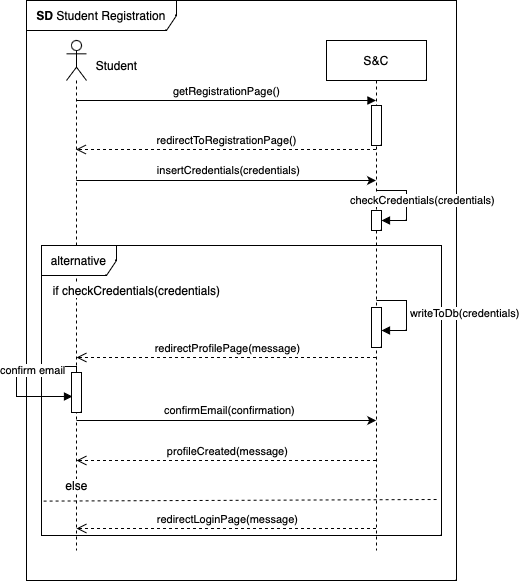
\includegraphics[width=1\textwidth]{RASD/Images/UseCases/StudentRegistration.drawio.png}
                \label{fig:example}
            \end{figure}

            % -- US5 --                                                      
            \newpage
            \item \textbf{Complete Student Profile}                         
            
            \begin{longtable}{|l|p{11cm}|}  
                \hline
                \textbf{Name} & 
                    \textbf{Complete Student Profile} \\
                \hline
                
                \textbf{Actors} & 
                    Student \\
                \hline
                
                \textbf{Entry Condition} & 
                    The student has an account, is logged in, and is on his homepage. \\
                \hline
                
                \textbf{Event Flow} &
                    \begin{enumerate}[label=\arabic*., itemsep=0.2em]
                        \item The student presses the "Edit Profile" button;
                        \item S\&C redirects the student to the personal profile page;
                        \item The student types the \textit{Basic Information} in the corresponding form field:
                        \begin{itemize}[label=\textbullet, itemsep=0em]
                            \item The student types the phone number;
                            \item The student uploads the profile picture;
                            \item The student enters the location for location-based internships.
                        \end{itemize}

                        \item The student types the \textit{Academic Information}:
                        \begin{itemize}[label=\textbullet, itemsep=0em]
                            \item University/college name;
                            \item Degree program;
                            \item Year of study;
                            \item GPA;
                            \item Relevant courses or projects;
                            \item Graduation year.
                        \end{itemize}

                        \item The student types the \textit{Skills and Expertise}:
                        \begin{itemize}[label=\textbullet, itemsep=0em]
                            \item Technical skills (e.g., programming languages, tools, software);
                            \item Soft skills (e.g., communication, teamwork, leadership);
                            \item Certifications.
                        \end{itemize}

                        \item The student types the \textit{Experience and Achievements}:
                        \begin{itemize}[label=\textbullet, itemsep=0em]
                            \item Previous internship or work experience;
                            \item Volunteer work or extracurricular activities;
                            \item Achievements (e.g., awards, competitions, publications).
                        \end{itemize}

                        \item The student types the \textit{Internship Preferences}:
                        \begin{itemize}[label=\textbullet, itemsep=0em]
                            \item Desired field or industry (e.g., tech, finance, marketing);
                            \item Preferred location (remote, specific cities, etc.);
                            \item Availability (full-time, part-time, duration of internship);
                            \item Desired start date.
                        \end{itemize}

                        \item The student uploads the \textit{CV};

                        \item The student enters the \textit{Portfolio/Projects}:
                        \begin{itemize}[label=\textbullet, itemsep=0em]
                            \item Links to personal projects, GitHub, personal website, or portfolios for creative roles.
                        \end{itemize}
                        
                        \item The student types the \textit{Languages Spoken}.
                        \item The student presses the "Apply Changes" button;
                        \item S\&C validates the data;
                        \item S\&C redirects the student to the homepage of S\&C.
                    \end{enumerate} \\
                \hline
                
                \textbf{Exit Condition} & 
                    The student's profile is successfully updated and saved in the system. \\
                \hline
                
                \textbf{Exceptions} &
                    \begin{enumerate}[label=\arabic*., itemsep=0.1em]
                        \item Missing Required Fields:
                            \begin{itemize}[label=\textbullet, itemsep=0em]
                                \item If any mandatory fields are left empty, S\&C will display an error message.
                            \end{itemize}
                        \item Invalid Data Format:
                            \begin{itemize}[label=\textbullet, itemsep=0em]
                                \item If the phone number format is invalid, an error message is displayed;
                                \item If the GPA is outside the valid range, the system prompts for correction.
                            \end{itemize}
                        \item Profile Picture Upload Failed:
                            \begin{itemize}[label=\textbullet, itemsep=0em]
                                \item S\&C displays an error if the file format is unsupported or the size exceeds limits.
                            \end{itemize}
                        \item CV Upload Failed:
                            \begin{itemize}[label=\textbullet, itemsep=0em]
                                \item S\&C prompts for a valid upload in case of failure.
                            \end{itemize}
                        \item System Validation Error:
                            \begin{itemize}[label=\textbullet, itemsep=0em]
                                \item Any inconsistency in the data (e.g., incorrect graduation year) triggers an error message.
                            \end{itemize}            
                    \end{enumerate} \\
                \hline
                
            \end{longtable}

            \newpage
            \begin{figure}[h!]
                \centering  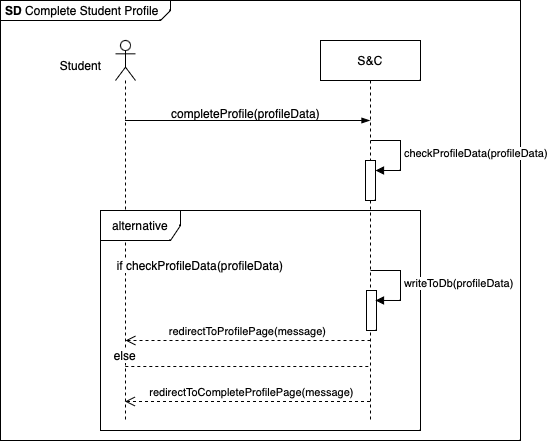
\includegraphics[width=1\textwidth]{RASD/Images/UseCases/CompleteProfile.drawio.png}
                \label{fig:CompleteStudentProfile}
            \end{figure}
            
            % -- US6 --
            \newpage
            \item \textbf{Internship Search}
            
            \begin{longtable}{|l|p{11cm}|}  
                \hline
                \textbf{Name} & 
                    \textbf{Internship Search} \\
                \hline
                
                \textbf{Actors} & 
                    Student \\
                \hline
               
                \textbf{Entry Condition} & 
                    \begin{enumerate}[label=\textbullet, itemsep=0em]
                        \item The student knows the search criteria;
                        \item The student has an account and is logged in.
                    \end{enumerate} \\
                \hline
                
                \textbf{Event Flow} &
                    \begin{enumerate}[label=\arabic*., itemsep=0.2em]
                        \item The student clicks on the "Search" button
                        \item S\&C redirects the student to the search page;
                        \item The student searches for keyword or compiles some filters options;
                        \item The student issues the search
                        \item S\&C looks for the results and shows them with a preview for each internship;
                        \item The student can now scroll the list of internships that match the search criteria;
                        \item If the student is interested in any of the shown positions can click to discover more about it;
                        %\item Included use case: Application for internship
                    \end{enumerate} \\
                \hline
                
                \textbf{Exit Condition} & 
                    The user leaves the search page by clicking any button redirecting him or her to another page of the website \\
                \hline
                
                \textbf{Exceptions} &
                    \begin{enumerate}[label=\arabic*., itemsep=0.1em]
                        \item The criteria do not match any open position
                            \begin{itemize}[label=\textbullet, itemsep=0em]
                                \item In that case, S\&C will redirect the student will show a notification on the screen saying that no open position matched the search criteria
                            \end{itemize}
                        \item One or more keywords entered are not valid.
                            \begin{itemize}[label=\textbullet, itemsep=0em]
                                \item In that case, S\&C will display an empty list and a warning message on the screen saying that the input keywords don't exist.
                            \end{itemize}
                    \end{enumerate} \\
                \hline
            \end{longtable}
            
            \newpage
            \begin{figure}[h!]
                \centering  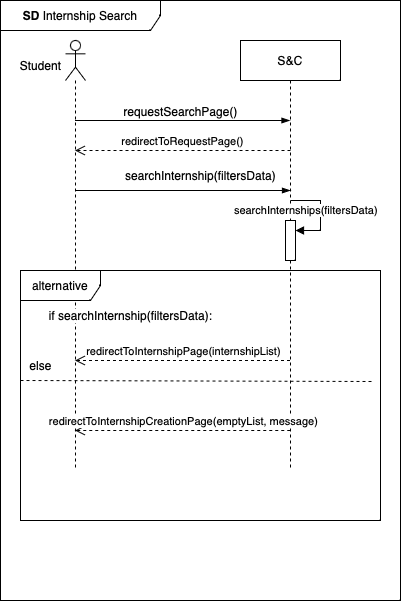
\includegraphics[]{RASD/Images/UseCases/InternshipSearch.drawio.png}
                \label{fig:CompleteStudentProfile}
            \end{figure}

            % -- US7 --
            \newpage
            \item \textbf{Application for internship}
            
            \begin{longtable}{|l|p{11cm}|}  
                \hline
                \textbf{Name} & 
                    \textbf{Application for Internship} \\
                \hline
                
                \textbf{Actors} & 
                    Student \\
                \hline
                
                \textbf{Entry Condition} & 
                    \begin{enumerate}[label=\textbullet, itemsep=0em]
                        \item The student decides to apply to an internship;
                        \item The student has an account and is logged in;
                        \item The student searched an internship and he/she is on the dedicated page.
                    \end{enumerate} \\
                \hline
                
                \textbf{Event Flow} &
                    \begin{enumerate}[label=\arabic*., itemsep=0.2em]
                        \item The student presses the "Apply" button;
                        \item S\&C redirects the student to the page of the internship position;
                        \item The student can see all the information
                        \item The student has to accept terms and condition of the application
                        \item The student presses the "Confirm" button
                    \end{enumerate} \\
                \hline
                
                \textbf{Exit Condition} & 
                    The user sent the application and gets redirected to his own profile page\\
                \hline
                
                \textbf{Exceptions} &
                    \begin{enumerate}[label=\arabic*., itemsep=0.1em]
                        \item One or more keywords entered are not valid.
                            \begin{itemize}[label=\textbullet, itemsep=0em]
                                \item In that case, S\&C will display an empty list and a warning message on the screen saying that the input keywords don't exist.
                            \end{itemize}
                    \end{enumerate} \\
                \hline
            \end{longtable}
    
            \newpage
            \begin{figure}[h!]
                \centering   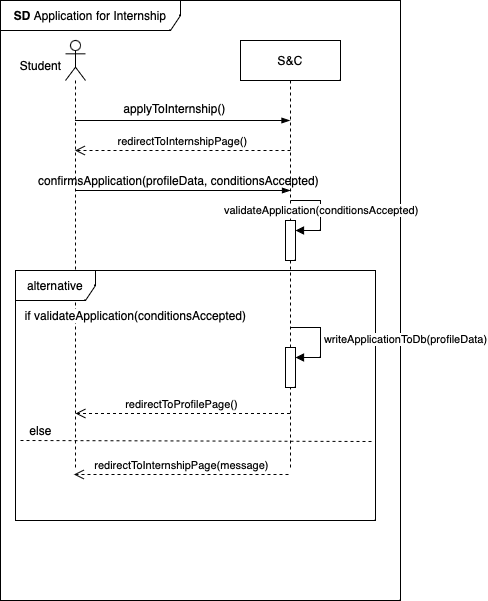
\includegraphics{RASD/Images/UseCases/InternshipApplication.drawio.png}
                \label{fig: Application for Internship}
            \end{figure}

        \end{enumerate}

    % -----------------------------------
    \newpage
    \subsubsection{Company Use Cases}
        \begin{enumerate}[label=\textbf{[US\arabic*]}, left = 0pt, align = left, resume]
            % -- US8 --
            \item \textbf{Company Registration}
        
            \begin{longtable}{|l|p{11cm}|}  
                \hline
                \textbf{Name} & 
                    \textbf{Company Registration} \\
                \hline
                
                \textbf{Actors} & 
                    Company \\
                \hline
                
                \textbf{Entry Condition} & 
                    The company does not have an account and is on the main page of S\&C. \\
                \hline
                
                \textbf{Event Flow} &
                    \begin{enumerate}[label=\arabic*., itemsep=0.2em]
                        \item The company presses the "Register as Company" button;
                        \item S\&C redirects the company to the register page;
                        \item The company types the company mail in the corresponding form field;
                        \item The company types the password in the corresponding form field;
                        \item The company types the confirm password in the corresponding form field;
                        \item The company types the its name in the corresponding form field;
                        \item The company presses the "Subscribe" button;
                        \item S\&C validates the data;
                        \item S\&C sends a confirmation email;
                        \item S\&C displays a success message (email sent);
                        \item The company enters its mailbox;
                        \item The company opens the mail sent by S\&C;
                        \item The company presses the "Confirm Registration" button in the email;
                        \item S\&C creates the company's account;
                        \item S\&C redirects the company to the homepage of S\&C.
                    \end{enumerate} \\
                \hline
                
                \textbf{Exit Condition} & 
                    The company's account is created, and it's logged in. \\
                \hline
                
                \textbf{Exceptions} &
                    \begin{enumerate}[label=\arabic*., itemsep=0.1em]
                        \item A user with the entered email already exists.
                            \begin{itemize}[label=\textbullet, itemsep=0em]
                                \item In that case, S\&C will redirect the company to the login page.
                            \end{itemize}
                        \item The email entered isn't valid.
                            \begin{itemize}[label=\textbullet, itemsep=0em]
                                \item In that case, S\&C will display an error message on the screen.
                            \end{itemize}
                        \item The password and the confirmation password do not match.
                            \begin{itemize}[label=\textbullet, itemsep=0em]
                                \item In that case, S\&C will display an error message on the screen.
                            \end{itemize}
                    \end{enumerate} \\
                \hline
                
            \end{longtable}

            \newpage
            \begin{figure}[h!]
                \centering  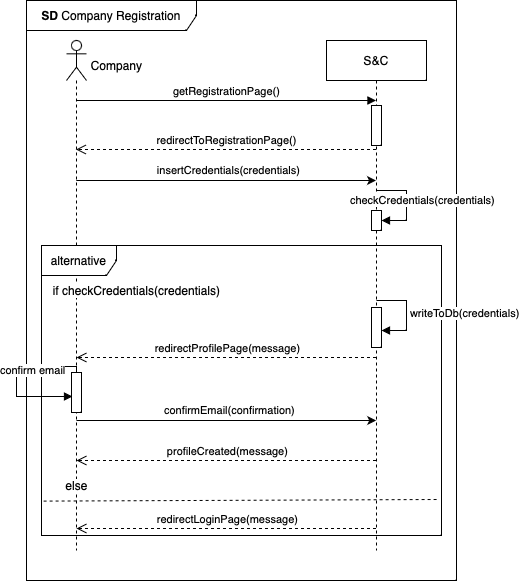
\includegraphics[width=1\textwidth]{RASD/Images/UseCases/CompanyRegistration.drawio.png}
                \label{fig:CompanyRegistration}
            \end{figure}

            % -- US9 --
            \newpage
            \item \textbf{Post a New Internship}
            
            \begin{longtable}{|l|p{11cm}|}  
                \hline
                \textbf{Name} & 
                    \textbf{Post a new internship} \\
                \hline
                
                \textbf{Actors} & 
                    Company \\
                \hline
                
                \textbf{Entry Condition} & 
                    The company has an account and is logged in. \\
                \hline
                
                \textbf{Event Flow} &
                    \begin{enumerate}[label=\arabic*., itemsep=0.2em]
                        \item The company presses the "Add New Internship" button;
                        \item S\&C displays a form that the company have to fill;
                        \item The company fills the form;
                        \item The company presses the "Publish" button;
                        \item S\&C validates the data;
                        \item S\&C displays a Success Message;
                        \item S\&C redirects the company to the main page;
                    \end{enumerate} \\
                \hline
                
                \textbf{Exit Condition} & 
                    The company posts a new internship. \\
                \hline
                
                \textbf{Exceptions} &
                    \begin{enumerate}[label=\arabic*., itemsep=0.1em]
                        \item The company leaves one or more mandatory fields empty.
                            \begin{itemize}[label=\textbullet, itemsep=0em]
                                \item S\&C displays an error message indicating the missing fields.
                                \item S\&C highlights the empty fields in the form.
                                \item The company is prompted to complete the form before resubmitting.
                            \end{itemize}
                        \item The company provides invalid data (e.g., incorrect date formats, non-numeric salary inputs).
                            \begin{itemize}[label=\textbullet, itemsep=0em]
                                \item S\&C validates the input and detects the invalid data.
                                \item S\&C displays an error message explaining the specific validation errors.
                                \item The company must correct the errors and resubmit the form
                            \end{itemize}
                        \item The company is not logged in.
                            \begin{itemize}[label=\textbullet, itemsep=0em]
                                \item S\&C denies access and displays an error message: "You must be logged in with a company account to perform this action."
                                \item S\&C redirects the user to the login page.
                            \end{itemize}
                        \item The company attempts to post an internship with identical details to an already existing one.
                            \begin{itemize}[label=\textbullet, itemsep=0em]
                                \item S\&C detects the duplicate entry and displays a warning: "An internship with similar details already exists. Please review your submission."
                            \end{itemize}
                    \end{enumerate} \\
                \hline
                
            \end{longtable}

            \newpage
            \begin{figure}[h!]
                \centering  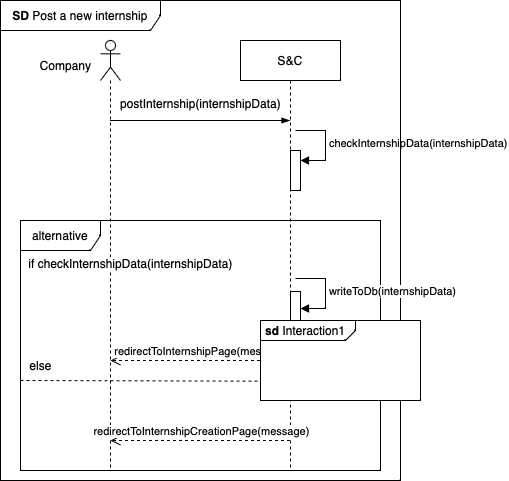
\includegraphics{RASD/Images/UseCases/PostNewInternship.drawio.png}
                \label{fig:example}
            \end{figure}

            % -- US10 --        % MODIFICATO
            \newpage
            \item \textbf{Close a new internship}
            
            \begin{longtable}{|l|p{11cm}|}  
                \hline
                \textbf{Name} & 
                    \textbf{Close a new internship} \\
                \hline
                
                \textbf{Actors} & 
                    Company \\
                \hline
                
                \textbf{Entry Condition} & 
                    \begin{enumerate}[label=\textbullet, itemsep=0em]
                        \item The company has an account and is logged in;
                        \item The company has at least one open internship.
                    \end{enumerate} \\
                \hline 
                
                \textbf{Event Flow} &
                    \begin{enumerate}[label=\arabic*., itemsep=0.2em]
                        \item The company enters the open internship section;
                        \item The company chooses the internship they want to close;
                        %\item The company fills the form;
                        \item The company presses the "Close" button;
                        %\item S\&C validates the data;
                        \item S\&C displays a Success Message;
                        \item S\&C redirects the company to the main page;
                    \end{enumerate} \\
                \hline
                
                \textbf{Exit Condition} & 
                    The company posts a new internship. \\
                \hline
                
                \textbf{Exceptions} &
                    \begin{enumerate}[label=\arabic*., itemsep=0.1em]
                        \item The company is not logged in.
                            \begin{itemize}[label=\textbullet, itemsep=0em]
                                \item S\&C denies access and displays an error message: "You must be logged in with a company account to perform this action."
                                \item S\&C redirects the user to the login page.
                            \end{itemize}
                    \end{enumerate} \\
                \hline
                
            \end{longtable}

            \newpage     % DA RIFARE CON MODIFICHE
            \begin{figure}[h!]
                \centering        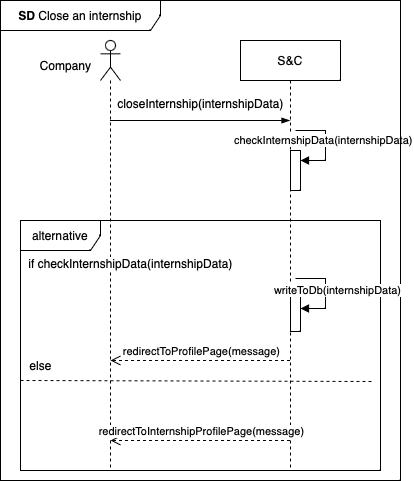
\includegraphics{RASD/Images/UseCases/CloseInternship.drawio.png}
                \label{fig:example}
            \end{figure}

            % -- US11 --        % MODIFICATO
            \newpage
            \item \textbf{Application Acceptance or Rejection}
            
            \begin{longtable}{|l|p{11cm}|}  
                \hline
                \textbf{Name} & 
                    \textbf{Application Acceptance or Rejection} \\
                \hline
                
                \textbf{Actors} & 
                    Company \\
                \hline
                
                \textbf{Entry Condition} & 
                    \begin{enumerate}[label=\textbullet, itemsep=0em]
                        \item The company has an account and is logged in;
                        \item The company knows which candidate to accept or reject. 
                    \end{enumerate} \\
                \hline
                
                \textbf{Event Flow} &
                    \begin{enumerate}[label=\arabic*., itemsep=0.2em]
                        \item The company goes to the page of an open internship it has;
                        \item The company clicks on the button to see the list of candidates;
                        \item The company can click on each item of the list to visit the profile page of the candidate;
                        \item The company clicks on the "Accept" or "Reject" button in correspondence with the candidate
                    \end{enumerate} \\
                \hline
                
                \textbf{Exit Condition} & 
                    The candidate is accepted or rejected. \\
                \hline
                
                \textbf{Exceptions} &
                    \begin{enumerate}[label=\arabic*., itemsep=0.1em]
                        \item The company has no candidates for an open internship.
                            \begin{itemize}[label=\textbullet, itemsep=0em]
                                \item In that case, S\&C will show an empty list an display a notification which says no applications were found for that position.
                            \end{itemize}
                    \end{enumerate} \\
                \hline
            \end{longtable}

            \newpage
            \begin{figure}[h!]
                \centering  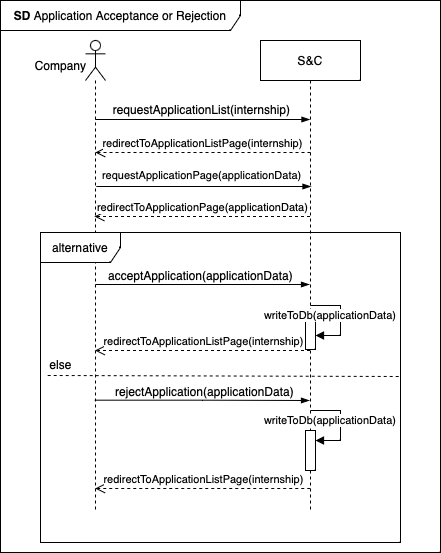
\includegraphics{RASD/Images/UseCases/ApplicationAcceptanceRejection.drawio.png}
                \label{fig:example}
            \end{figure}

            % -- US12 --
            \newpage
            \item \textbf{Further Assessment for Application}
            
            \begin{longtable}{|l|p{11cm}|}  
                \hline
                \textbf{Name} & 
                    \textbf{Further Assessment for Application} \\
                \hline
                
                \textbf{Actors} & 
                    Company\\
                \hline
                
                \textbf{Entry Condition} & 
                    \begin{enumerate}[label=\textbullet, itemsep=0em]
                        \item The company has an account and is logged in;
                        \item The company knows which candidates have to undergo more assessment before being accepted or rejected.
                    \end{enumerate} \\
                \hline
                
                \textbf{Event Flow} &
                    \begin{enumerate}[label=\arabic*., itemsep=0.2em]
                        \item The company goes to the page of an open internship it has;
                        \item The company clicks on the button to see the list of candidates;
                        \item The company can click on each item of the list to visit the profile page of the candidate;
                        \item The company clicks the "Assess Further" button in correspondence with the candidate
                        \item The company is prompted a calendar to choose when to schedule the interview and an input field to put the link of the online room
                        \item The company confirms the date
                        
                    \end{enumerate} \\
                \hline
                
                \textbf{Exit Condition} & 
                    The company is redirected to its profile page \\
                \hline
                
                \textbf{Exceptions} &
                    \begin{enumerate}[label=\arabic*., itemsep=0.1em]
                        \item The company has no candidates for an open internship.
                            \begin{itemize}[label=\textbullet, itemsep=0em]
                                \item In that case, S\&C will show an empty list and display a notification which says no applications were found for that position.
                                \end{itemize}                           
                                \item The company inserted the wrong link.
                                \begin{itemize}[label=\textbullet, itemsep=0em]
                                \item In that case, the company will have to inform the student with a different communication mean (e. g. by email)
                                \end{itemize}
                    \end{enumerate} \\
                \hline
            \end{longtable}
            
            \newpage
            \begin{figure}[h!]
                \centering  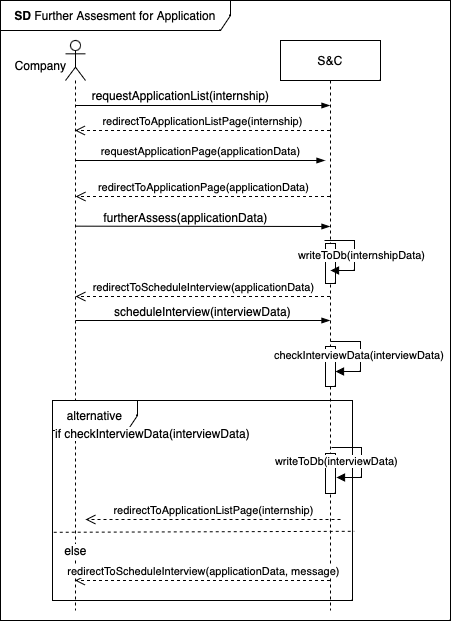
\includegraphics{RASD/Images/UseCases/FurtherAssessment.drawio.png}
                \label{fig:example}
            \end{figure}
            
        \end{enumerate}

    % -----------------------------------
    \newpage
    \subsubsection{Users (Company and Student) Use Cases}
    Notice that in this subsection when we refer to users we intend students and companies only.
        \begin{enumerate}[label=\textbf{[US\arabic*]}, left = 0pt, align = left, resume]
            % -- US13 --
            \item \textbf{Feedback from User}
            
            \begin{longtable}{|l|p{11cm}|}  
                \hline
                \textbf{Name} & 
                    \textbf{Feedback from User} \\
                \hline
                
                \textbf{Actors} & 
                    User\\
                \hline
                
                \textbf{Entry Condition} & 
                    \begin{enumerate}[label=\textbullet, itemsep=0em]
                        \item The user has an account and is logged in;
                        \item The user has participated in the internship;
                        \item The internship has finished.
                    \end{enumerate} \\
                \hline
                
                \textbf{Event Flow} &
                    \begin{enumerate}[label=\arabic*., itemsep=0.2em]
                        \item The user navigates to the page of the just finished internship;
                        \item The user clicks the button to create a feedback;
                        \item The user inserts a rating and a comment;
                        \item The user sends it by clicking "Send" 
                    \end{enumerate} \\
                \hline
                
                \textbf{Exit Condition} & 
                    The feedback is sent and the user is redirected to the application page \\
                \hline
                \hline
            \end{longtable}

            \begin{figure}[h!]
                \centering  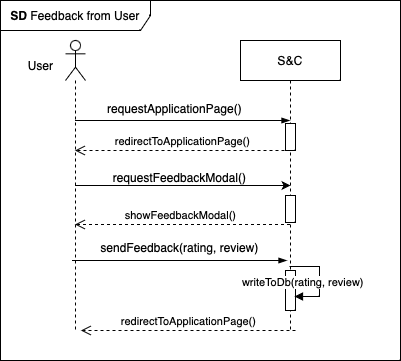
\includegraphics{RASD/Images/UseCases/FeedbackFromUser.drawio.png}
                \label{fig:example}
            \end{figure}

            % -- US14 --
            \newpage
            \item \textbf{Communication between Users}
            
            \begin{longtable}{|l|p{11cm}|}  
                \hline
                \textbf{Name} & 
                    \textbf{Feedback from Student/Company} \\
                \hline
                
                \textbf{Actors} & 
                    User\\
                \hline
                
                \textbf{Entry Condition} & 
                    \begin{enumerate}[label=\textbullet, itemsep=0em]
                        \item The user has an account and is logged in;
                        \item The user is participating in the internship;
                        \item A user has to communicate something while an internship is ongoing.
                    \end{enumerate} \\
                \hline
                
                \textbf{Event Flow} &
                    \begin{enumerate}[label=\arabic*., itemsep=0.2em]
                        \item The user navigates to the page of the ongoing internship;
                        \item The user clicks the button to create a new message;
                        \item The user inserts a message and sends it; 
                    \end{enumerate} \\
                \hline
                
                \textbf{Exit Condition} & 
                    The message is sent and the student/company is redirected to the application page \\
                \hline
                \hline
            \end{longtable}

            \begin{figure}[h!]
                \centering        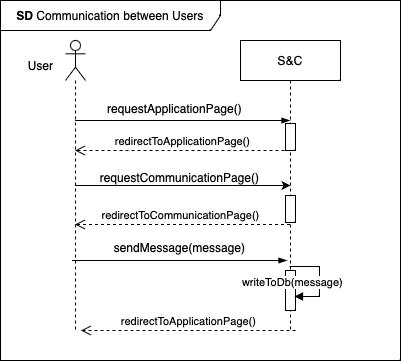
\includegraphics{RASD/Images/UseCases/CommunicationBetweenUsers.drawio.png}
                \label{fig:example}
            \end{figure}

        \end{enumerate}

    % -----------------------------------
    \newpage
    \subsubsection{Universities Use Cases}
        \begin{enumerate}[label=\textbf{[US\arabic*]}, left = 0pt, align = left, resume]
            % -- US15 --
            \item \textbf{University Monitors Internships}
            
            \begin{longtable}{|l|p{11cm}|}  
                \hline
                \textbf{Name} & 
                    \textbf{University Monitors Internships} \\
                \hline
                
                \textbf{Actors} & 
                    University \\
                \hline
                
                \textbf{Entry Condition} & 
                    The university is logged in \\
                \hline
                
                \textbf{Event Flow} &
                    \begin{enumerate}[label=\arabic*., itemsep=0.2em]
                        \item The university has a list of internships done by its students on its home page;
                        \item The university can click on any of them to get more details;
                    \end{enumerate} \\
                \hline
                
                \textbf{Exit Condition} & 
                    The university stops scrolling the list of hits students who got an internship  profile. \\
                \hline
                
                \textbf{Exceptions} &
                    \begin{enumerate}[label=\arabic*., itemsep=0.1em]
                        \item The universities has no students who got an internship.
                            \begin{itemize}[label=\textbullet, itemsep=0em]
                                \item In that case, S\&C will display a message on the screen saying that no enrolled student got any internship.
                            \end{itemize}
                    \end{enumerate} \\
                \hline
                
            \end{longtable}
            
            \begin{figure}[h!]
                \centering        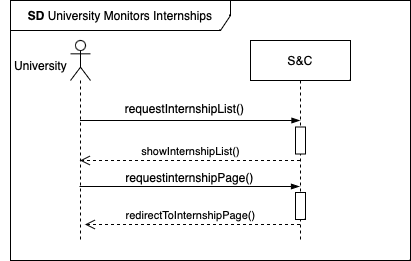
\includegraphics{RASD/Images/UseCases/UniversityMonitorsInternships.drawio.png}
                \label{fig:example}
            \end{figure}

        \end{enumerate}
            
% I merged the 2 use cases into 1
            % % -- US16 --
            % \item \textbf{Further Assessment for Application}
            
            % \begin{longtable}{|l|p{11cm}|}  
            %     \hline
            %     \textbf{Name} & 
            %         \textbf{Further Assessment for Application} \\
            %     \hline
                
            %     \textbf{Actors} & 
            %         Company\\
            %     \hline
                
            %     \textbf{Entry Condition} & 
            %         The company knows which candidates have to undergo more assessment before being accepted or rejected \\
            %     \hline
                
            %     \textbf{Event Flow} &
            %         \begin{enumerate}[label=\arabic*., itemsep=0.2em]
            %             \item Included use case: Company Login
            %             \item The company goes to the page of an open internship it has;
            %             \item The company clicks on the button to see the list of candidates;
            %             \item The company can click on each item of the list to visit the profile page of the candidate;
            %             \item The company clicks "Assess Further" 
            %             \item Included use case: Create assessment 
            %         \end{enumerate} \\
            %     \hline
                
            %     \textbf{Exit Condition} & 
            %         The candidate is notified that he has to undergo a phase of assessment. \\
            %     \hline
                
            %     \textbf{Exceptions} &
            %         \begin{enumerate}[label=\arabic*., itemsep=0.1em]
            %             \item The company has no candidates for an open internship.
            %                 \begin{itemize}[label=\textbullet, itemsep=0em]
            %                     \item In that case, S\&C will show an empty list and display a notification which says no applications were found for that position.
            %                 \end{itemize}
            %         \end{enumerate} \\
            %     \hline
            % \end{longtable}

            % % -- US17 --
            % \newpage
            % \item \textbf{Request Assessment}
            
            % \begin{longtable}{|l|p{11cm}|}  
            %     \hline
            %     \textbf{Name} & 
            %         \textbf{Request Assessment} \\
            %     \hline
                
            %     \textbf{Actors} & 
            %         Company, Student\\
            %     \hline
                
            %     \textbf{Entry Condition} & 
            %         The company pressed the button "Request Assessment" on an application \\
            %     \hline
                
            %     \textbf{Event Flow} &
            %         \begin{enumerate}[label=\arabic*., itemsep=0.2em]
            %             \item The company is prompted a calendar to choose when to schedule the interview and an input field to put the link of the online room
            %             \item After confirming the decision, the company is redirected to the page of the internship needing the assessment;
            %             \item From now on it will be able to accept or reject the student;
            %             \item The company clicks "Create Assessment" 
            %         \end{enumerate} \\
            %     \hline
                
            %     \textbf{Exit Condition} & 
            %         The assessment for the student has been created. \\
            %     \hline
                
            %     \textbf{Exceptions} &
            %         \begin{enumerate}[label=\arabic*., itemsep=0.1em]
            %             \item The company inputs the wrong date.
            %                 \begin{itemize}[label=\textbullet, itemsep=0em]
            %                     \item In that case, the company will have to inform the student with a different communication mean (e. g. by email)
            %                 \end{itemize}
            %             \item The company inserted the wrong link.
            %             \begin{itemize}[label=\textbullet, itemsep=0em]
            %             \item In that case, the company will have to inform the student with a different communication mean (e. g. by email)
            %             \end{itemize}
            %         \end{enumerate} \\
            %     \hline
            % \end{longtable}
